\chapter{多态}

\section{多态}

\subsection{多态(Polymorphism)}

多态是同一个行为具有多个不同表现形式或形态的能力。

\begin{figure}[H]
	\centering
	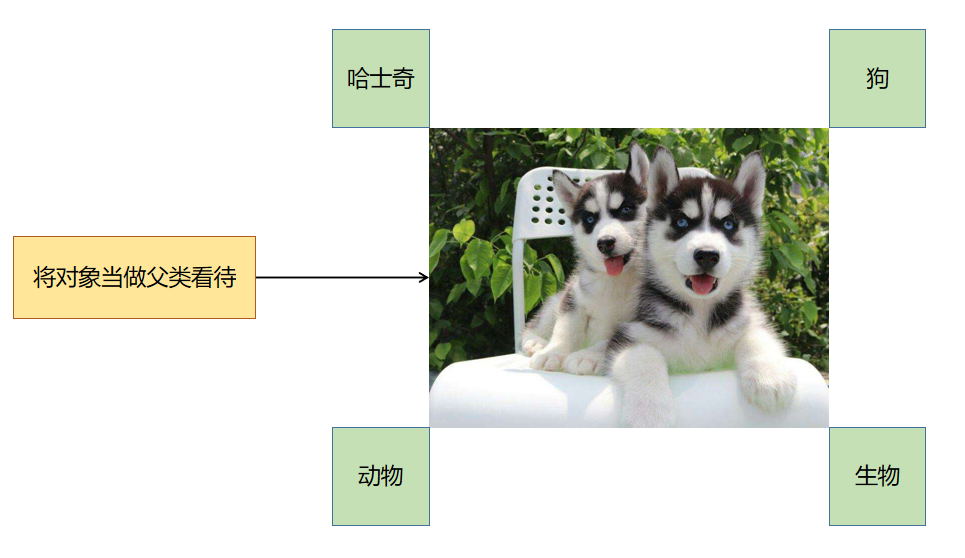
\includegraphics[scale=0.7]{img/C9/9-1/1.png}
	\caption{多态}
\end{figure}

\begin{figure}[H]
	\centering
	\begin{tikzpicture}[]
		\draw (0,0) node {Animal animal = new Dog();};

		\draw (-3,-2) rectangle (-1,-1);
		\draw (1,-2) rectangle (3,-1);
		\draw (-2,-1.5) node {父类引用};
		\draw (2,-1.5) node {子类对象};

		\draw[->] (-2,-1) -- (-1.5,-0.3);
		\draw[->] (2,-1) -- (1.5,-0.3);
	\end{tikzpicture}
	\caption{父类引用指向子类对象}
\end{figure}

通过父类引用指向子类对象,从而产生多种形态。父类引用仅能访问父类所声明的属性和方法,不能访问子类独有的属性和方法。 \\

在一对有继承关系的类中都有一个方法,其方法名、参数列表、返回值均相同,通过调用方法实现不同类对象完成不同的事件。

\newpage

\section{抽象类}

\subsection{抽象类(Abstract Class)}

抽象类不能被用于实例化对象,只是提供了所有的子类共有的部分。例如在动物园中,存在的都是“动物”具体的子类对象,并不存在“动物”对象,所以动物类不应该被独立创建成对象。 \\

抽象类的作用是可以被子类继承,提供共性的属性和方法。

\subsection{抽象方法(Abstract Method)}

父类提供的方法很难满足子类不同的需求,如果不定义该方法,则表示所有的子类都不具有该行为。如果定义该方法,所有的子类都在重写,那么这个方法在父类中是没有必要实现的,显得多余。 \\

被abstract关键字修饰的方法称为抽象方法。抽象方法只有声明,没有实现。抽象方法只能包含在抽象类中。产生继承关系后,子类必须重写父类中所有的抽象方法,否则子类还是抽象类。 \\

非抽象类在继承自一个抽象父类的同时,必须重写实现父类中所有的抽象方法。因此,抽象类可以用来做一些简单的规则制定。在抽象类中制定一些规则,要求所有的子类必须实现,约束所有子类的行为。 \\

但是,类是单继承的,一个类有且只能有一个父类,所以如果一个类需要受到多种规则的约束,无法再继承其它父类。此时可以使用接口进行这样的复杂的规则制定。

\newpage

\section{对象转型}

\subsection{对象转型}

对象由子类类型转型为父类类型,即是向上转型。向上转型是一种隐式转换,一定会转型成功。向上转型后的对象,只能访问父类中定义的成员。 \\

由父类类型转型转型为子类类型,即是向下转型。向下转型存在失败的可能性,会出现ClassCastException异常。向下转型需要进行强制类型转换,是一个显式转换。向下转型后的对象,将可以访问子类中独有的成员。 \\

向下转型存在失败的可能性。如果引用实际指向的对象,不是要转型的类型,此时强制转换会出现ClassCastException异常。所以,在向下转型之前,最好使用instanceof关键字进行类型检查。 \\

\mybox{对象转型}

\begin{lstlisting}[language=Java, title=Animal.java]
public abstract class Animal {
    private String name;

    public Animal(String name) {
        this.name = name;
    }

    public abstract void makeSound();
}
\end{lstlisting}

\begin{lstlisting}[language=Java, title=Dog.java]
public class Dog extends Animal {
    public Dog(String name) {
        super(name);
    }
    
    @Override
    public void makeSound() {
        System.out.println("汪汪~");
    }
}
\end{lstlisting}

\begin{lstlisting}[language=Java, title=TestDog.java]
public class TestDog {
    public static void main(String[] args) {
        Animal animal = new Dog("狗子");
        if(animal instanceof Dog) {
            Dog dog = (Dog)animal;
            dog.makeSound();
        }
    }
}
\end{lstlisting}

\begin{tcolorbox}
	\mybox{运行结果}
	\begin{verbatim}
汪汪~
	\end{verbatim}
\end{tcolorbox}

\newpage

\section{接口}

\subsection{接口}

在面向对象中会使用抽象类为外部提供一个通用的、标准化的接口。 \\

宏观上来讲,接口是一种标准。例如常见的USB接口,电脑通过USB接口连接各种外设设备,每一个接口不用关心连接的外设设备是什么,只要这个外设设备实现了USB的标准,就可以连接到电脑上。

\begin{figure}[H]
	\centering
	
\includegraphics[scale=0.4]{img/C9/9-4/1.png}
	\caption{USB接口}
\end{figure}

从程序上来讲,接口代表了某种能力和约定。当父类的方法无法满足子类需求时,可实现接口扩充子类的能力,接口中方法的定义代表能力的具体要求。 \\

定义接口需要使用关键字interface,接口中可以定义:

\begin{enumerate}
	\item 属性:默认都是静态常量,访问权限都是public。
	\item 方法:默认都是抽象方法,访问权限都是public。
\end{enumerate}

接口和抽象类的相同点有:

\begin{enumerate}
	\item 都不能创建对象。
	\item 都具备Object类中所定义的方法。
	\item 都可以写抽象方法。
\end{enumerate}

接口和抽象类的不同点有:

\begin{enumerate}
	\item 接口中所有的属性都是公开静态常量,缺省用public static final修饰。
	\item 接口中所有的方法都是公开抽象方法,缺省用public abstract修饰。
	\item 接口中没有构造方法、构造代码段和静态代码段。
\end{enumerate}

因为接口中有很多抽象方法,因此非抽象类在实现接口的时候必须重写实现接口中所有的抽象方法。 \\

使用接口可以进行对行为的约束和规则的制定,接口表示一组能力,那么一个类可以接受多种能力的约束。因此一个类可以实现多个接口,实现多个接口的时候,必须要把每一个接口中的方法都实现。如果一个类实现的多个接口中有相同的方法,实现类只需实现一次即可。 \\

\mybox{接口}

\begin{lstlisting}[language=Java, title=USB.java]
public interface USB {
    /**
     * USB接口返回当前连接设备的类型
     * @return 当前连接设备
     */
    String getDeviceInfo();
}
\end{lstlisting}

\begin{lstlisting}[language=Java, title=Mouse.java]
public class Mouse implements USB {
    @Override
    public String getDeviceInfo() {
        return "mouse";
    }
}
\end{lstlisting}

\begin{lstlisting}[language=Java, title=Keyboard.java]
public class Keyboard implements USB {
    @Override
    public String getDeviceInfo() {
        return "keyboard";
    }
}
\end{lstlisting}

\begin{lstlisting}[language=Java, title=Computer.java]
public class Computer {
    // 电脑有2个USB接口
    private USB usb1;
    private USB usb2;
    
    public void setUsb1(USB usb1) {
        this.usb1 = usb1;
    }
    
    public void setUsb2(USB usb2) {
        this.usb2 = usb2;
    }
    
    /**
     * 获取USB接口连接设备的信息
     */
    public String getUsbInfo() {
        return "USB 1: " + this.usb1.getDeviceInfo() + "\n"
                + "USB 2: " + this.usb2.getDeviceInfo();
    }
}
\end{lstlisting}

\begin{lstlisting}[language=Java, title=TestUsb.java]
public class TestUsb {
    public static void main(String[] args) {
        Computer computer = new Computer();
        
        // 外设设备连接到电脑上
        computer.setUsb1(new Mouse());
        computer.setUsb2(new Keyboard());
        
        System.out.println(computer.getUsbInfo());
    }
}
\end{lstlisting}

\begin{tcolorbox}
	\mybox{运行结果}
	\begin{verbatim}
USB 1: mouse
USB 2: keyboard
	\end{verbatim}
\end{tcolorbox}

\newpage